\documentclass[10pt,a4paper]{article}
\usepackage[T1]{fontenc}
\usepackage[utf8]{inputenc}
\usepackage{lmodern}
\usepackage{microtype}
\usepackage[margin=2cm]{geometry}
\usepackage{amsmath}
\usepackage{booktabs}
\usepackage{graphicx}
\usepackage{caption}
\usepackage[hidelinks]{hyperref}
\usepackage{xurl}
\graphicspath{{../figures/}{../figures/png/}{figures/}{figures/png/}}   % residual_length, rf_residual, horizon_residual (PDF or PNG)

\captionsetup{font=small,labelfont=bf}
\setlength{\parskip}{3pt plus 1pt}
\setlength{\parindent}{0pt}
\setlength{\textfloatsep}{8pt plus 2pt minus 2pt}
\renewcommand{\arraystretch}{1.05}

\title{24-hour-ahead electricity load forecasting: recurrent vs.\ convolutional networks and the role of seasonal baselines}
\author{}   % add names
\date{}

\begin{document}
\maketitle

\begin{abstract}
I compare LSTM, GRU and temporal convolutional networks (TCN) of matched size, plus a simplified CNN-GRU hybrid, for one-shot 24-hour-ahead forecasting of 10 clients of the UCI ElectricityLoadDiagrams20112014 data. Trained directly, all networks are worse than the trivial forecast ``repeat last week'' (MAE 16.5--17.9~kW against 14.4~kW). Letting the network predict only a correction to last week's load removes the gap; the residual TCN is then reliably better than the residual GRU (0.52~kW, paired 95\% CI [0.21, 0.94]) but its advantage over last week's load is small and concentrated in a few days. A plain average of the same hours over the last four weeks is better than last week's load and at least as accurate as every learned model I trained, including networks trained to correct that average. Longer inputs, L1 loss and the hybrid give no reliable benefit. The main lesson is methodological: against a strong seasonal baseline and with paired, day-level uncertainty, most architecture differences vanish.
\end{abstract}

\section{Introduction}
Electricity load has strong daily and weekly cycles, so a one-day-ahead forecast benefits from information up to a week or more back. Bai et al.\ \cite{bai} argue that generic convolutional networks (TCN) match or beat recurrent networks on sequence tasks, and Lai et al.\ \cite{lai} discuss why recurrent models struggle with long periodic patterns on this same dataset. I revisit that comparison on the UCI data \cite{uci} with a one-shot 24~h forecast, and ask whether the networks add anything beyond simple seasonal forecasts.

My contributions, in the order the work developed:
\begin{enumerate}\itemsep0pt
  \item A negative baseline result: with the standard setup, all three networks lose to ``repeat last week'' (Section~\ref{sec:direct}).
  \item A residual formulation in which the network predicts only a correction to a seasonal forecast, and a comparison of anchors: last week's load and the four-week mean (Sections~\ref{sec:direct}, \ref{sec:length}).
  \item Stronger non-learned baselines (multi-week averages) and a paired, day-level evaluation with block-bootstrap intervals, which changes several conclusions that the mean MAE alone would suggest (Sections~\ref{sec:paired}--\ref{sec:mean4}).
  \item A test of the hybrid design suggested by the assignment, a simplified convolution + recurrence model inspired by LSTNet \cite{lai}, which brings no gain over a GRU (Section~\ref{sec:paired}).
\end{enumerate}

\section{Methods and materials}
\textbf{Data.} I use 10 of the 370 clients (MT\_156, 159, 169, 232, 242, 248, 266, 281, 302, 307), drawn once with a fixed seed among clients with no zero-load hours since 2012 (\texttt{configs/clients.json}). The 15-minute readings are averaged to hourly values. The series from 2012-01-01 is split chronologically 70/10/20 into train/validation/test (the test period runs from late May to December 2014); z-scoring uses training statistics only and windows never cross split boundaries. Validation and test windows start at midnight, so every forecast covers one calendar day.

\textbf{Task and metrics.} Input: the last $L$ hours of all 10 clients ($L \times 10$). Output: the next 24 hours of all clients in one shot ($24 \times 10$), from a linear head on the last time step. Metrics are computed in kW: MAE (primary) and RMSE, plus WAPE per client (client MAE divided by its mean load). The October 2014 clock change doubles one 01:00 hour; a secondary ``noDST'' MAE excludes the two affected days, and changes the MAEs of the paired-analysis runs by at most 0.05~kW.

\textbf{Models} (about 68k parameters each, so capacity is comparable): LSTM, 2 layers $\times$ 64 units (68,336 parameters); GRU, 2 layers $\times$ 72 units (67,200); TCN, 7 residual blocks of two weight-normalised causal dilated convolutions, kernel 3, dilations $1,2,\dots,64$, 38 channels (68,298; receptive field $1+4(2^n-1)=509$~h), written from scratch following \cite{bai}. Training: Adam (learning rate $10^{-3}$, halved on validation plateau), batch 64, MSE on normalised data, gradient clipping 1.0, dropout 0.1, at most 40 epochs, early stopping with patience 6. Every configuration is trained with 5 seeds.

\textbf{Residual variants.} The network output is added to a seasonal forecast taken from the input window, so the network only learns a correction: either the same 24 hours one week earlier (needs $L\ge168$), or their mean over the last four weeks (\texttt{residual: mean4}, needs $L\ge672$).

\textbf{Hybrid (CNN-GRU).} Inspired by the convolution + recurrence design of LSTNet \cite{lai}, but a simplified model of my own: two causal convolutions (kernel 6, 32 channels, ReLU, dropout) with a $1\times1$ skip from the input, read by a 2-layer GRU (64 units), same head (67,856 parameters). It is not LSTNet: I omit its skip-recurrent component and its autoregressive highway; the seasonal residual plays a similar role to the highway but is a different mechanism.

\textbf{Baselines.} naive-24h (yesterday); naive-168h (same day last week); mean-2w, mean-4w and median-4w (mean or median of the same 24 hours over the last 2 or 4 weeks). The four-week baselines need 672~h of history.

\textbf{Paired evaluation.} A window needs $L$ hours of history inside the test split, so a model with input length $L$ is scored on days starting $L$ hours into the test period: $L=672$ sees 21 fewer days (191 vs 212) than $L=168$, and mean MAEs across $L$ are computed on different days. All comparisons that matter are therefore made on the days both models cover. For a model and a reference I report the mean daily MAE difference (diff = reference minus model, so positive favours the model; averaged over seeds), a 95\% interval from a moving-block bootstrap (7-day blocks, because daily errors are autocorrelated), the share of days on which the model wins, and the range over seeds. These runs are retrained with forecasts saved and can differ slightly from the mean tables (e.g.\ 13.68 vs 13.52~kW for the TCN with L1 at $L=672$), by about the seed spread. The intervals describe the single test period, not other years or clients.

\textbf{Reproducibility.} All configurations are generated by \texttt{scripts/make\_configs.py}; \texttt{README.md} lists the commands for training (\texttt{src.train}), the tables (\texttt{src.plots}) and the paired analysis (\texttt{src.analyze}).

\section{Results}

\subsection{Direct forecasts lose to last week; the residual formulation closes the gap}\label{sec:direct}
\begin{table}[h]
\centering\footnotesize
\caption{Test MAE [kW], $L=168$, mean $\pm$ standard deviation over 5 seeds.}
\begin{tabular}{@{}lcccc@{}}
\toprule
 & direct, MSE & direct, L1 & residual, MSE & residual, L1\\
\midrule
LSTM    & $17.87\pm0.45$ & --              & --              & --\\
GRU     & $16.49\pm0.25$ & $16.12\pm0.29$  & $14.49\pm0.13$  & $14.50\pm0.20$\\
TCN     & $16.58\pm0.34$ & $16.42\pm0.24$  & $13.87\pm0.13$  & $13.79\pm0.15$\\
CNN-GRU & $17.14\pm0.39$ & --              & $14.48\pm0.09$  & --\\
\bottomrule
\end{tabular}
\end{table}

For reference, naive-24h has MAE 14.46 and naive-168h 14.43~kW (RMSE 30.7 and 28.3). Every directly trained network is worse than naive-168h; the LSTM is worst, GRU and TCN are indistinguishable. The gap is concentrated in client MT\_159 (mean load 44~kW; WAPE 45--55\% for the direct models against 30\% for naive-168h). L1 loss helps the direct models slightly. The residual formulation helps far more: the GRU reaches the level of naive-168h and the TCN has a lower mean MAE by about 0.55~kW. Training is also faster with the residual (GRU: 9 epochs against 19). Section~\ref{sec:paired} shows how much of the TCN's mean gain is reliable.

\subsection{Paired comparison over test days}\label{sec:paired}
\begin{table}[h]
\centering\footnotesize
\caption{Paired comparison on common test days. diff = reference MAE $-$ model MAE [kW] (positive: model better); CI: 95\% moving-block bootstrap; ``better'': share of days on which the model wins.}\label{tab:paired}
\begin{tabular}{@{}llrrcrl@{}}
\toprule
model & reference & days & diff & 95\% CI & better & per-seed diff\\
\midrule
GRU (res, L168)      & naive-168h       & 212 & $-0.06$ & [$-0.26$, 0.18]  & 43\% & $-0.29$ .. 0.11\\
TCN (res, L168)      & naive-168h       & 212 & 0.46    & [0.02, 1.07]     & 47\% & 0.28 .. 0.54\\
TCN (res+L1, L672)   & naive-168h       & 191 & 0.31    & [$-0.03$, 0.69]  & 48\% & 0.18 .. 0.48\\
TCN (res, L168)      & GRU (res, L168)  & 212 & 0.52    & [0.21, 0.94]     & 58\% & 0.35 .. 0.60\\
TCN (res+L1, L672)   & GRU (res, L168)  & 191 & 0.45    & [0.18, 0.75]     & 60\% & 0.32 .. 0.62\\
CNN-GRU (res, L168)  & GRU (res, L168)  & 212 & 0.01    & [$-0.14$, 0.15]  & 50\% & $-0.16$ .. 0.11\\
CNN-GRU (res, L168)  & TCN (res, L168)  & 212 & $-0.51$ & [$-0.92$, $-0.20$] & 40\% & $-0.68$ .. $-0.41$\\
\bottomrule
\end{tabular}
\end{table}

The residual GRU is indistinguishable from naive-168h. The residual TCN is better than the residual GRU, with an interval that excludes zero and wins on 58--60\% of days: this is the one architecture effect that survives the paired test. Against naive-168h the TCN's mean gain barely excludes zero ($L=168$) or includes it ($L=672$ with L1), and the TCN is better on fewer than half of the days. The gain is concentrated: for the $L=168$ TCN the median daily difference is $-0.06$~kW, and the mean gain falls from 0.46 to 0.12~kW when the ten days with the largest gains are removed. Those days lie mostly in 12--21 June 2014 (14 June: naive-168h 30.5~kW, TCN 15.4~kW), where repeating the previous week fails; I did not investigate the cause (a holiday or one-off event is plausible). The TCN is worse on 26 December (7.7~kW against 0.2~kW).

The hybrid is statistically identical to the GRU and clearly worse than the TCN: adding a convolutional front-end to a GRU does not reproduce the TCN's advantage.

\subsection{Input length and receptive field}\label{sec:length}
Residual test MAE [kW] by input length is given in Table~\ref{tab:length} and Figure~\ref{fig:length}; the plain-model sweep (not shown) likewise has no systematic benefit.

\begin{table}[h]
\centering\footnotesize
\caption{Residual models, test MAE [kW] by input length.}\label{tab:length}
\begin{tabular}{@{}lccc@{}}
\toprule
residual model & $L=168$ & $L=336$ & $L=672$\\
\midrule
GRU     & $14.49\pm0.13$ & $14.54\pm0.09$ & $14.55\pm0.40$\\
TCN     & $13.87\pm0.13$ & $14.20\pm0.20$ & $14.02\pm0.20$\\
CNN-GRU & $14.48\pm0.09$ & $14.69\pm0.14$ & $14.55\pm0.32$\\
\bottomrule
\end{tabular}
\end{table}

\begin{figure}[h]
\centering
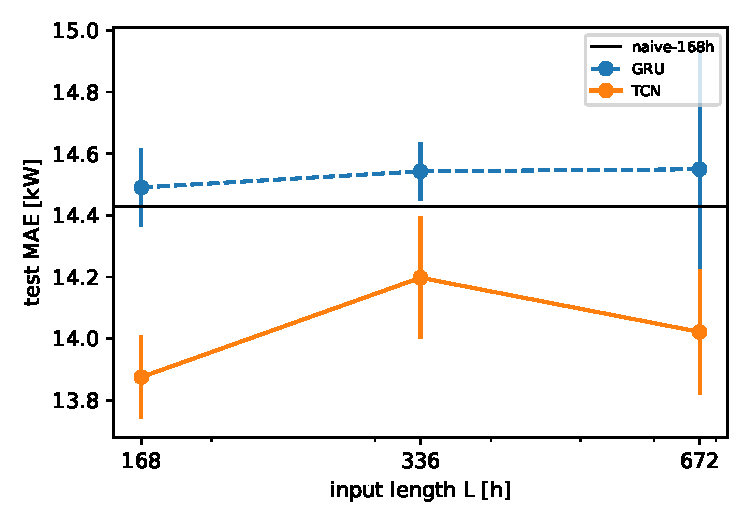
\includegraphics[width=0.58\linewidth]{residual_length}
\caption{Test MAE of the residual models by input length (squares: with L1 loss; dotted: CNN-GRU; horizontal line: naive-168h).}\label{fig:length}
\end{figure}

Longer inputs do not help. On common days the residual GRU at $L=672$ is worse than at $L=168$ ($-0.42$~kW, CI [$-0.71$, $-0.03$]) and worse than naive-168h ($-0.56$, [$-0.94$, $-0.07$]); the residual TCN at $L=336$ is slightly worse than at $L=168$ ($-0.20$, [$-0.38$, $-0.04$]). The TCN with L1 loss at $L=672$ has the lowest mean MAE (13.52), but against the $L=168$ TCN the difference is $+0.14$~kW, CI [$-0.05$, 0.30]; since it also changes the loss, it does not isolate an effect of $L$. I therefore do not claim that a longer input or L1 loss improves the TCN: one week of history is the best or equal-best input length.

Receptive field (Figure~\ref{fig:rf}; residual TCN, $L=672$, $n=3,\dots,8$ blocks, receptive field 29, 61, 125, 253, 509, 1021~h): MAE 14.47, 14.38, 14.37, \textbf{14.00}, 14.02, 14.03~kW (standard deviation 0.08--0.31). The error is flat, close to naive-168h, while the receptive field is shorter than one week, drops by about 0.37~kW once it exceeds 168~h, and does not improve further. The hidden width is fixed, so the parameter count grows with depth (33k to 77k); the plateau from $n=6$ to 8 occurs while the parameter count still grows by 30\%, so capacity alone does not explain the step. The pattern is consistent with the network needing to see the same hours of the previous week to learn useful corrections, but I did not test this further.

\begin{figure}[h]
\centering
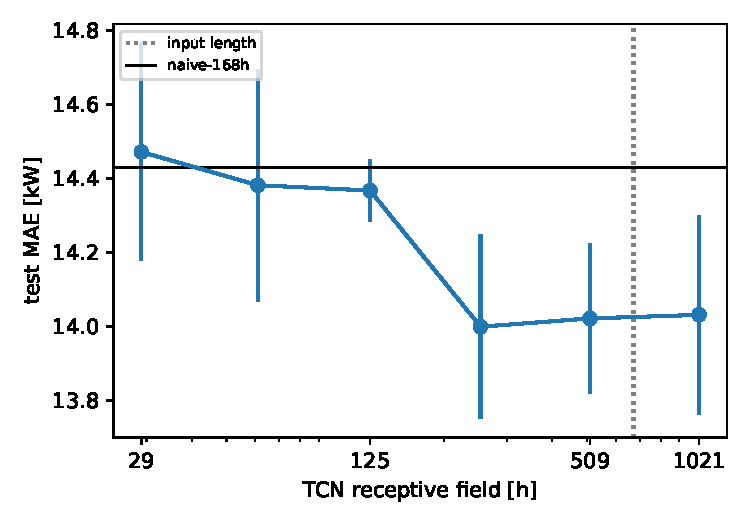
\includegraphics[width=0.58\linewidth]{rf_residual}
\caption{Test MAE of the residual TCN against its receptive field ($L=672$). Dotted vertical line: input length; horizontal line: naive-168h.}\label{fig:rf}
\end{figure}

\subsection{A multi-week average is at least as good as the learned models}\label{sec:mean4}
\begin{table}[h]
\centering\footnotesize
\caption{Multi-week baseline and learned models on the 191 common days (same conventions as Table~\ref{tab:paired}).}
\begin{tabular}{@{}llrcr@{}}
\toprule
model & reference & diff [kW] & 95\% CI & better\\
\midrule
mean-4w                              & naive-168h & 0.76    & [0.14, 1.42]       & 60\%\\
TCN (res, L168)                      & mean-4w    & $-0.59$ & [$-1.17$, 0.01]    & 39\%\\
TCN (res+L1, L672)                   & mean-4w    & $-0.45$ & [$-1.04$, 0.15]    & 42\%\\
GRU (res, L168)                      & mean-4w    & $-0.90$ & [$-1.56$, $-0.28$] & 38\%\\
TCN (res on mean-4w, L672)           & mean-4w    & $-0.47$ & [$-0.83$, $-0.00$] & 39\%\\
TCN (res on mean-4w + L1, L672)      & mean-4w    & $-0.31$ & [$-0.71$, 0.17]    & 37\%\\
GRU (res on mean-4w, L672)           & mean-4w    & $-0.67$ & [$-1.15$, $-0.02$] & 35\%\\
\bottomrule
\end{tabular}
\end{table}

On the 191 days that all models cover, mean-4w has MAE 13.23~kW, against 13.68 for the best learned model in the paired runs (TCN, residual + L1, $L=672$). It improves on naive-168h by 0.76~kW; mean-2w ($+0.49$) and median-4w ($+0.69$) behave similarly. Averaging removes the noise of one atypical week, the failure mode seen in June 2014. No learned model is better than mean-4w: the intervals of the TCNs include or barely exclude zero, and the GRU is clearly worse. I also trained the networks to correct mean-4w itself (\texttt{residual: mean4}, $L=672$); their MAE is 13.70 (TCN), 13.54 (TCN + L1) and 13.90~kW (GRU) against 13.23, and the learned correction does not improve on the TCN anchored to last week ($+0.28$~kW, CI [$-0.38$, 0.97]). The correction therefore adds error instead of removing it (mean-4w is exactly the network with a correction of zero). On the validation days the picture is different: the mean squared error of mean-4w is 0.125 (normalised units, 80 days), whereas the selected networks reach 0.116, about 7\% lower, while on the test days they are worse than mean-4w (RMSE excluding the two clock-change days: 25.8--26.3~kW against 25.4~kW). This is consistent with overfitting to the period used for model selection, or with a shift between validation and test period, but it is weak evidence: early stopping picks the best validation epoch, so the validation figure is optimistic, and 80 days are few. Seed spread is large (up to 1.5~kW against mean-4w for one TCN seed), so single runs are unreliable.

\subsection{Per client and per forecast hour}
\begin{table}[h]
\centering\footnotesize
\caption{WAPE [\%] per client (best of the five methods in bold). *: scored on the 191-day period, the others on 212 days.}
\begin{tabular}{@{}lrccccc@{}}
\toprule
client & mean load [kW] & naive-24h & naive-168h & mean-4w* & GRU (res) & TCN (res)\\
\midrule
MT\_156 &  89 & 24.5 & 14.4 & \textbf{12.0} & 14.7 & 14.3\\
MT\_159 &  44 & 48.5 & 30.0 & \textbf{26.8} & 30.8 & 33.2\\
MT\_169 &  43 &  5.9 &  6.8 & \textbf{5.8}  &  6.7 &  6.3\\
MT\_232 &  82 & \textbf{6.2} & 7.6 & 6.6 &  7.6 &  7.3\\
MT\_242 & 178 & \textbf{6.7} & 8.1 & 7.9 &  8.5 &  8.3\\
MT\_248 & 155 & \textbf{5.0} & 6.3 & 5.5 &  6.2 &  5.7\\
MT\_266 & 268 & \textbf{6.3} & 7.2 & 6.7 &  7.2 &  7.0\\
MT\_281 & 111 & \textbf{4.7} & 5.8 & 5.5 &  5.8 &  5.6\\
MT\_302 & 117 & \textbf{5.0} & 6.4 & 7.0 &  6.3 &  5.9\\
MT\_307 & 767 & \textbf{6.0} & 6.8 & 6.1 &  6.7 &  6.3\\
\bottomrule
\end{tabular}
\end{table}

The two irregular clients (MT\_156, MT\_159) have by far the largest relative errors for every model, and they are where averaging over weeks helps most. ``Repeat yesterday'' has a lower WAPE than every learned model on 8 of the 10 clients (all but MT\_156 and MT\_159), and the lowest of all methods on 7 of them, but is much worse on the two irregular clients, so its pooled MAE equals naive-168h. All residual models are anchored to last week; for clients with a weak weekly cycle this anchor is worse than yesterday and the networks do not fully compensate. The pooled kW MAE also weights clients by load (MT\_307 alone contributes about a third), so per-client relative errors and pooled errors can rank methods differently. Per forecast hour (Figure~\ref{fig:hour}) all models and baselines share the same shape: errors are lowest at night (forecast hours 2--6, about 10~kW) and peak in the afternoon (16--17~kW), so differences between methods are small compared with the variation over the day.

\begin{figure}[h]
\centering
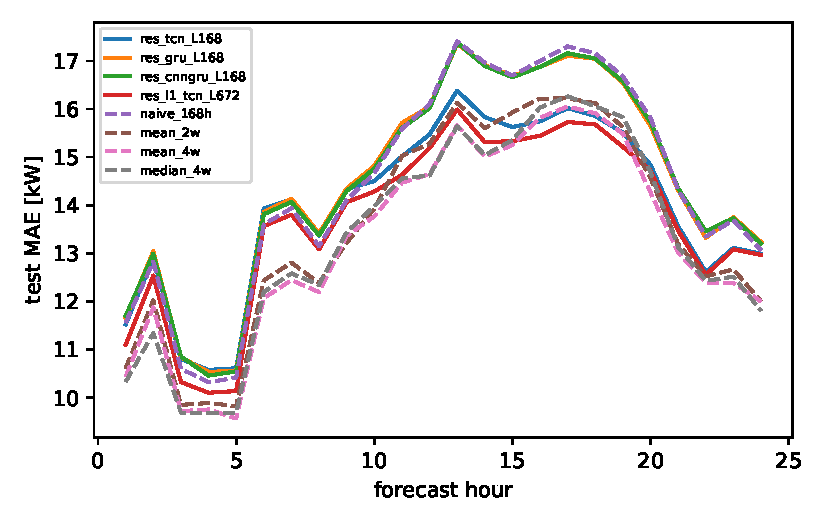
\includegraphics[width=0.58\linewidth]{horizon_residual}
\caption{Test MAE by forecast hour. Solid: learned models; dashed: seasonal baselines (mean-2w, mean-4w, median-4w on 191 days, naive-168h on 212 days).}\label{fig:hour}
\end{figure}

\section{Discussion}
\textbf{Why do direct networks lose?} Naive-168h is a strong baseline because load is dominated by weekly repetition. A direct network must reconstruct last week's values from normalised inputs through a bottleneck (the last hidden state or time step, 38--72 units) before the head, which costs accuracy on the part of the signal that is easiest to predict; the residual formulation hands that part over directly. This is plausible but not isolated by my experiments: the benefit may also come from the easier optimisation of a low-variance target.

\textbf{Recurrent vs.\ convolutional.} Without the residual I do not reproduce a clear advantage of the TCN over the GRU as reported in \cite{bai}, although the LSTM is worst. With the residual the TCN is reliably better than the GRU. It is not the longer window that produces this ($L=168$ is as good as longer inputs); the step in the receptive-field experiment suggests that covering one week matters. The advantage may come from the convolutional inductive bias on the correction signal, or from capacity and optimisation; I did not separate these. The hybrid shows that the gain is not simply ``convolutions help'', and since it omits LSTNet's skip-recurrent and highway components, my result is no evidence against the full LSTNet \cite{lai}. Numbers are not comparable with \cite{lai}, which uses other clients, splits and metrics.

\textbf{What do the networks add?} Little, in this setting. Past load is largely explained by its weekly (and multi-week average) profile; the corrections the networks learn do not reliably beat a four-week average, even when they are trained directly on it. This is a finding for the tested configurations and period, not a general claim that neural networks cannot improve on seasonal averages.

\textbf{Limitations.} Only 10 clients and a single chronological split (about 200 test days), so conclusions may depend on the test period; one hyperparameter setting per architecture, with capacity matched by parameter count rather than tuned; models see past load only, with no calendar, holiday or weather inputs, which probably handicaps the direct networks (not tested); training windows start at every hour but test windows at midnight, which may cost the direct models accuracy (not tested); the June 2014 gain concentration was not traced to a cause. Future work: rolling-origin evaluation over several periods, more clients, calendar and weather covariates, an equal tuning budget, and learned models that combine several seasonal anchors.

\section{Conclusion}
Directly trained LSTM, GRU and TCN forecasters lose to ``repeat last week'' for 24-hour-ahead load of 10 clients. Predicting a correction to last week's load removes the gap and makes the TCN reliably better than the GRU, but the TCN's advantage over the seasonal baseline is small and rests on a few days, and a four-week average is at least as accurate as every learned model I trained, including a convolution + recurrence hybrid, longer inputs, L1 loss and networks trained to correct the average. For this task, a strong seasonal baseline and paired, day-level evaluation matter more than the choice of architecture.

\begin{thebibliography}{3}
\bibitem{bai} S. Bai, J. Z. Kolter, and V. Koltun, ``An empirical evaluation of generic convolutional and recurrent networks for sequence modeling,'' arXiv:1803.01271, 2018.
\bibitem{lai} G. Lai, W.-C. Chang, Y. Yang, and H. Liu, ``Modeling long- and short-term temporal patterns with deep neural networks,'' in \emph{Proc.\ 41st Int.\ ACM SIGIR Conf.\ Research and Development in Information Retrieval}, 2018.
\bibitem{uci} A. Trindade, ``ElectricityLoadDiagrams20112014,'' UCI Machine Learning Repository, 2015. [Online]. Available: \url{https://doi.org/10.24432/C58C86}
\end{thebibliography}

\end{document}
